% This is the TU Munich LaTeX template, optimized for R Markdown.

% -------------------------------
% --- PREAMBLE ---
% -------------------------------
\documentclass[a4paper]{article}
\usepackage{geometry}
\usepackage{amsmath,amssymb,amsfonts,amsthm}    % Typical maths resource packages
\usepackage{graphicx}                           % Packages to allow inclusion of graphics
\usepackage[authoryear]{natbib}                 % literature reference style
\usepackage[bf]{caption}                        % For caption
\usepackage{textcomp}                           % For single quotes
\usepackage{floatrow}                           % For image and table position
\usepackage[notransparent]{svg}                 % For image in SVG
\usepackage{booktabs}                           % For tables
\usepackage{tabularx}                           % For tables
\usepackage{pifont}                             % For special marks
\usepackage{longtable}                          % For long tables
\usepackage{diagbox}                            % For tables diagbox
\usepackage[colorlinks=true, linkcolor=black]{hyperref}      % For creating hyperlinks in cross references
\usepackage[bottom, flushmargin]{footmisc}                   % For footnotes                        

% -------------------------------
% --- some layout definitions ---
% -------------------------------

% define topline
\usepackage[automark]{scrlayer-scrpage}
\pagestyle{scrheadings}
\automark{section}
\clearscrheadings
\ohead{\headmark}

% define citation style
%\bibliographystyle{ecta}
%\bibliographystyle{apacite}

% define page size, margin size
\geometry{top=2.35cm, left=2.5cm, right=2.5cm, bottom=2.35cm, includehead, includefoot}
\setcounter{secnumdepth}{3}
\setcounter{tocdepth}{3}   

% define line spacing = 1.5
\renewcommand{\baselinestretch}{1.5}

% define font size in footnotes = 10 pt
\renewcommand\footnotelayout{\fontsize{10}{12}\selectfont}

% define position of graphics
\floatsetup[figure]{capposition=bottom}
\floatsetup[table]{capposition=top}
\floatplacement{figure}{ht}   
\floatplacement{table}{ht}

% save thesis parameters for later
\newcommand{\thesistype}{TYPE OF THE WORK}
\newcommand{\thesisauthor}{NAME}
\newcommand{\thesisdate}{SUBMISSION DATE}

% define tightlist to work with newer versions of pandoc
\providecommand{\tightlist}{%
  \setlength{\itemsep}{0pt}\setlength{\parskip}{0pt}}

% change spacing
\setlength {\parskip}{1em}

% create TUM logo
\newcommand{\bildklein}[3]{  
	\begin{figure}[hp]
	\begin{center}
	\includegraphics[width=0.5\textwidth]{#1}
	\end{center}
	\caption[#2]{#3}
	\end{figure}
}
  	
\newcommand{\bildgross}[3]{  
	\begin{figure}[hp]
	\begin{center}
	\includegraphics[width=0.95\textwidth]{#1}
	\end{center}
	\caption[#2]{#3}
	\end{figure}
}
  

\newcommand{\eqn}[3]{
	\begin{figure}[hp]
	\begin{equation}#1\end{equation}
	\caption[#2]{#3}
	\end{figure}
}

% This is tumlogo.tex
%
% Neues TUM-Logo in TeX
%   by G. Teege, 19.10.89
% Benutzung:
%   Am Anfang des Dokuments (TeX oder LaTeX):
%     \input tumlogo
%   Dann beliebig oft:
%     \TUM{<breite>}
%   bzw.
%     \oTUM{<breite>}
%   \TUM setzt das Logo mit der Breite <breite> und der entsprechenden Hoehe.
%   <breite> muss eine <dimen> sein. \oTUM erzeugt eine "outline"-Version
%   des Logos, d.h. weiss mit schwarzem Rand. Bei \TUM ist es ganz schwarz.
%   \oTUM entspricht damit der offiziellen Version des Logos.
%   Das Logo kann wie ein einzelnes Zeichen verwendet werden.
%   Beispiel:
%     Dies ist das TUM-Logo: \oTUM{1cm}.
%
\def\TUM#1{%
\dimen1=#1\dimen1=.1143\dimen1%
\dimen2=#1\dimen2=.419\dimen2%
\dimen3=#1\dimen3=.0857\dimen3%
\dimen4=\dimen1\advance\dimen4 by\dimen2%
\setbox0=\vbox{\hrule width\dimen3 height\dimen1 depth0pt\vskip\dimen2}%
\setbox1=\vbox{\hrule width\dimen1 height\dimen4 depth0pt}%
\setbox2=\vbox{\hrule width\dimen3 height\dimen1 depth0pt}%
\setbox3=\hbox{\copy0\copy1\copy0\copy1\box2\copy1\copy0\copy1\box0\box1}%
\leavevmode\vbox{\box3}}
%
\def\oTUM#1{%
\dimen1=#1\dimen1=.1143\dimen1%
\dimen2=#1\dimen2=.419\dimen2%
\dimen3=#1\dimen3=.0857\dimen3%
\dimen0=#1\dimen0=.018\dimen0%
\dimen4=\dimen1\advance\dimen4 by-\dimen0%
\setbox1=\vbox{\hrule width\dimen0 height\dimen4 depth0pt}%
\advance\dimen4 by\dimen2%
\setbox8=\vbox{\hrule width\dimen0 height\dimen4 depth0pt}%
\advance\dimen4 by-\dimen2\advance\dimen4 by-\dimen0%
\setbox4=\vbox{\hrule width\dimen4 height\dimen0 depth0pt}%
\advance\dimen4 by\dimen1\advance\dimen4 by\dimen3%
\setbox6=\vbox{\hrule width\dimen4 height\dimen0 depth0pt}%
\advance\dimen4 by\dimen3\advance\dimen4 by\dimen0%
\setbox9=\vbox{\hrule width\dimen4 height\dimen0 depth0pt}%
\advance\dimen4 by\dimen1%
\setbox7=\vbox{\hrule width\dimen4 height\dimen0 depth0pt}%
\dimen4=\dimen3%
\setbox5=\vbox{\hrule width\dimen4 height\dimen0 depth0pt}%
\advance\dimen4 by-\dimen0%
\setbox2=\vbox{\hrule width\dimen4 height\dimen0 depth0pt}%
\dimen4=\dimen2\advance\dimen4 by\dimen0%
\setbox3=\vbox{\hrule width\dimen0 height\dimen4 depth0pt}%
\setbox0=\vbox{\hbox{\box9\lower\dimen2\copy3\lower\dimen2\copy5%
\lower\dimen2\copy3\box7}\kern-\dimen2\nointerlineskip%
\hbox{\raise\dimen2\box1\raise\dimen2\box2\copy3\copy4\copy3%
\raise\dimen2\copy5\copy3\box6\copy3\raise\dimen2\copy5\copy3\copy4\copy3%
\raise\dimen2\box5\box3\box4\box8}}%
\leavevmode\box0}
% End of tumlogo.tex



% Additional LaTeX parameters added in the YAML header of index.Rmd
  \usepackage{float}
  \floatplacement{figure}{H}

% --------------------------------------
% --------------------------------------
% --------------------------------------
% --- the structure the tex document ---
% frontmatter:
%   - cover,
%   - titlepage,
%   - acknowledgement,
%   - abstract,
%   - table of contents,
%   - list of figures,
%   - list of tables,
%   - list of abbreviations.
%
% body of the thesis:
%   - introduction,
%   - related work,
%   - hypotheses development,
%   - data collection,
%   - methods,
%   - results,
%   - discussion,
%   - conclusion,
%   - literature,
%   - appendix (figures, tables).
%
% --------------------------------------
% --------------------------------------
% --------------------------------------
\begin{document}
% -------------------------------
% --- frontmatter: Cover -
% -------------------------------
\thispagestyle{empty}
\begin{center}
	\bigskip \bigskip \bigskip 
	\oTUM{4.0cm} \\
	\vspace*{1cm}
	{ \bf FAKULTÄT FÜR INFORMATIK} \\
	{ \bf DER TECHNISCHEN UNIVERSITÄT MÜNCHEN} \\
	\bigskip \bigskip \bigskip \bigskip \bigskip
	{ TYPE OF THE WORK} \\
	\bigskip \bigskip \bigskip \bigskip \bigskip
	\bigskip \bigskip \bigskip \bigskip \bigskip
	{\Large \bf TITLE} \\        
	\bigskip \bigskip \bigskip \bigskip
	{\Large NAME} \\    
	\bigskip\bigskip \bigskip \bigskip
	\begin{figure}[ht]
	\centering 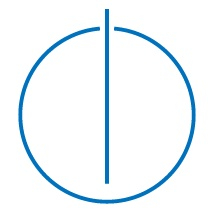
\includegraphics[width=0.2\linewidth]{infologo.jpg}
	\end{figure}
	\bigskip 
\end{center}
\vfill

% -------------------------------
% --- frontmatter: Title page   -
% -------------------------------
\newpage
\thispagestyle{empty}
\begin{center}
	\bigskip \bigskip \bigskip 
	\oTUM{4.0cm} \\
	\vspace*{1cm}
	{ \bf FAKULTÄT FÜR INFORMATIK} \\
	{ \bf DER TECHNISCHEN UNIVERSITÄT MÜNCHEN} \\
	\bigskip \bigskip \bigskip
	{TYPE OF THE WORK} \\
	\bigskip \bigskip \bigskip
	{\Large \bf TITLE} \\        
	\bigskip \bigskip \bigskip
	{\Large \bf TITLE IN GERMAN} \\
	\bigskip \bigskip \bigskip
\end{center}
\begin{table}
\centering
\begin{tabular}{ll}
{Author:} & {NAME} \\
{Supervisor:} & {NAME OF PROFESSOR} \\
{Advisor:} & {NAME OF ADVISOR} \\
{Submission:} & {SUBMISSION DATE} \\
\end{tabular}
\end{table}
\begin{figure}[ht]
	\centering 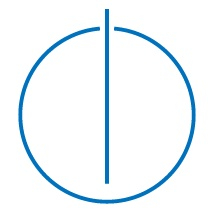
\includegraphics[width=0.2\linewidth]{infologo.jpg}
\end{figure}
\vfill

% -------------------------------
% --- Declaration ---------------
% -------------------------------
\newpage	
\thispagestyle{empty}
\vspace*{\fill}
\noindent I confirm that this master's thesis is my own work and I have documented all sources and material used.\\\\
\vspace{1cm}

München,

\vspace{3cm}

. . . . . . . . . . . . . . . . . . . . . . . . . . . . . . .
\vspace{0.1cm}

\thesisauthor{}

% ------------------------------------
% --- frontmatter: Acknowledgement ---
% ------------------------------------
\newpage
\hypertarget{acknowledgements}{%
\section*{Acknowledgements}\label{acknowledgements}}
\addcontentsline{toc}{section}{Acknowledgements}
\pagestyle{plain}
\clearpairofpagestyles
\ofoot*{\fontsize{8pt}{0pt}\pagemark} % font size for page number = 8pt
\pagenumbering{roman}   % define page number in roman style
\setcounter{page}{1}    % start page numbering

% -----------------------------
% --- frontmatter: Abstract ---
% -----------------------------
\newpage
\hypertarget{abstract}{%
\section*{Abstract}\label{abstract}}
\addcontentsline{toc}{section}{Abstract}

% -----------------------------
% --- frontmatter: Contents ---
% -----------------------------
\newpage
\tableofcontents
\clearpage

% ----------------------------------------------------
% --- frontmatter: List of Figures (not mandatory) ---
% ----------------------------------------------------
\newpage
\listoffigures
\addcontentsline{toc}{section}{List of Figures}

% ---------------------------------------------------
% --- frontmatter: List of Tables (not mandatory) ---
% ---------------------------------------------------
\newpage
\listoftables
\addcontentsline{toc}{section}{List of Tables}

% ----------------------------------------------------------
% --- frontmatter: List of Abbreviations (not mandatory) ---
% ----------------------------------------------------------
\newpage
\hypertarget{list-of-abbreviations}{%
\section*{List of Abbreviations}\label{list-of-abbreviations}}
\addcontentsline{toc}{section}{List of Abbreviations}

% -------------------------------
% --- main body of the thesis ---
% -------------------------------
\newpage
\pagestyle{scrplain}  
\clearpairofpagestyles
\ofoot*{\fontsize{8pt}{0pt}\pagemark} % font size for page number = 8pt
\setcounter{page}{1}    % start page numbering
\pagenumbering{arabic}  % page numbers in arabic style

\hypertarget{introduction}{%
\section{Introduction}\label{introduction}}

\newpage

\hypertarget{related-work}{%
\section{Related Work}\label{related-work}}

\newpage

\hypertarget{hypotheses-development}{%
\section{Hypotheses Development}\label{hypotheses-development}}

\newpage

\hypertarget{data-collection}{%
\section{Data Collection}\label{data-collection}}

\newpage

\hypertarget{methods}{%
\section{Methods}\label{methods}}

\newpage

\hypertarget{results}{%
\section{Results}\label{results}}

\newpage

\hypertarget{discussion}{%
\section{Discussion}\label{discussion}}

\newpage

\hypertarget{conclusion}{%
\section{Conclusion}\label{conclusion}}

\newpage

\hypertarget{references}{%
\section*{References}\label{references}}
\addcontentsline{toc}{section}{References}

\noindent

\setlength{\parindent}{-0.5cm}
\setlength{\leftskip}{0.5cm}
\setlength{\parskip}{8pt}

\hypertarget{refs}{}

\indent
\setlength{\parindent}{17pt}
\setlength{\leftskip}{0pt}
\setlength{\parskip}{0pt}

\newpage

\appendix

\hypertarget{appendix}{%
\section{Appendix}\label{appendix}}

\hypertarget{figures}{%
\subsection{Figures}\label{figures}}

\hypertarget{tables}{%
\subsection{Tables}\label{tables}}

% change rmd_files in `_bookdown.yml` files to determine order
% note that references and appendix are also contained here.

\end{document}
